\documentclass[aspectratio=169,11pt]{beamer}
\usepackage[T1]{fontenc}\usepackage{lmodern}\usepackage{booktabs}\usepackage{array}
\usepackage{tikz}\usetikzlibrary{arrows.meta,positioning,shapes.geometric}
\usepackage{xcolor}
\definecolor{NITNavy}{RGB}{18,42,76}\definecolor{NITBlue}{RGB}{39,91,145}\definecolor{NITLight}{RGB}{232,241,250}
\setbeamercolor{frametitle}{fg=NITNavy}\setbeamercolor{structure}{fg=NITBlue}\setbeamertemplate{navigation symbols}{}
\setbeamertemplate{footline}{\hfill\insertframenumber\hspace{0.5cm}\vspace{0.15cm}}
\setbeamertemplate{frametitle}{\vspace{.18cm}\begin{beamercolorbox}[wd=\paperwidth,sep=.12cm,leftskip=.55cm]{frametitle}\insertframetitle\end{beamercolorbox}\vspace{-.05cm}\hspace{.55cm}\rule{.91\paperwidth}{.6pt}}
\newcommand{\NITHeader}{\begin{center}{\large\bfseries National Institute of Technology Tiruchirappalli}\\[-1mm]{\normalsize\bfseries Department of Computer Science and Engineering}\end{center}\vspace{-2mm}\hrule\vspace{3mm}}
\title{Evolutionary, Generative AI and Graph Learning for Fraud Detection in Healthcare Insurance Claims}
\author{Thirilokkiyan K\\Roll No.: 206125028\\Guide: Dr. C. Mala}
\date{}
\begin{document}
\begin{frame}\NITHeader\titlepage\end{frame}

\begin{frame}{Introduction}
\begin{itemize}
\item Healthcare fraud is a major global problem; traditional rule-based/manual detection struggles with evolving fraud.
\item Key ML challenges: high-dimensional claims data and severe class imbalance.
\item WOA/GA can support feature selection and hyperparameter optimization; GAN/LLM methods can address minority-class scarcity.
\item Graph learning models relationships among providers, beneficiaries, diagnoses, procedures and time rather than treating records independently.
\end{itemize}\end{frame}

\begin{frame}{Literature Survey -- Including MHGSL}\scriptsize
\begin{tabular}{p{.05\textwidth}p{.31\textwidth}p{.25\textwidth}p{.31\textwidth}}\toprule
\textbf{S.No.}&\textbf{Paper Details}&\textbf{Techniques Used}&\textbf{Gaps Identified}\\\midrule
1&Nabrawi \& Alanazi, \emph{Risks}, 2023&RF; LR; ANN&No high-dimensionality handling; limited optimization.\\
2&Tubishat et al., \emph{Knowledge-Based Systems}, 2025&DW-WOA-SVM; dynamic search; LLM synthetic data&Nested-CV cost; synthetic-data realism; WOA-family focus.\\
3&Cai et al., \emph{Information}, 2026&WCGAN-GP; GA; RF&Precision--recall trade-off; single regional dataset; GAN cost.\\
4&Hong et al., \emph{Health insurance fraud detection based on multi-channel heterogeneous graph structure learning}, \emph{Heliyon}, 2024&MHGSL; topology/feature/semantic graphs; multi-channel GCN; attention&Medical-A/B confidential; XAI/reason-level explanations not central.\\
5&Sowah et al., \emph{J. Eng.}, 2019&GA + SVM&Limited Ghana dataset; no dynamic search.\\
6&Mao et al., 2024&GAN oversampling + XGBoost&Mode-collapse/training stability; no feature selection.\\
\bottomrule\end{tabular}\end{frame}

\begin{frame}{MHGSL -- Key Architecture}
\begin{columns}[T]
\column{.31\textwidth}\begin{block}{Heterogeneous Graph}Patients, departments, medicines and time with multiple relations.\end{block}
\column{.31\textwidth}\begin{block}{Three Views}Topology, feature-KNN and semantic meta-path graphs.\end{block}
\column{.31\textwidth}\begin{block}{Multi-Channel GCN}Specific and shared-parameter channels produce six embeddings; attention fuses them.\end{block}
\end{columns}
\begin{itemize}
\item Final representation $Z$ is used for classification/anomaly detection.
\item The paper combines cross-entropy with difference and consistency constraints.
\item Downstream experiments include RF, LR and XGBoost.
\end{itemize}\end{frame}

\begin{frame}{Dataset Selection for the Proposed Project}
\begin{block}{Recommended: Healthcare Provider Fraud Detection Analysis}
Public Kaggle dataset with linked Beneficiary, Inpatient, Outpatient and Provider-label files.
\end{block}
\begin{itemize}
\item 5,410 providers: 506 PotentialFraud=Yes and 4,904 No ($\approx9.35\%$ positive).
\item Beneficiary data includes demographics, chronic conditions and coverage.
\item Inpatient/outpatient claims include dates, provider IDs, diagnoses, procedures and reimbursement-related information.
\item The linked structure is suitable for a heterogeneous graph.
\end{itemize}
\end{frame}

\begin{frame}{MHGSL Dataset vs Proposed Public Dataset}\scriptsize
\begin{tabular}{p{.17\textwidth}p{.28\textwidth}p{.28\textwidth}p{.22\textwidth}}\toprule
\textbf{Aspect}&\textbf{MHGSL}&\textbf{Proposed dataset}&\textbf{Adaptation}\\\midrule
Target&Patient fraud/anomaly&Provider potential fraud&Provider target node\\
Entities&Patient, Department, Medicine, Time&Provider, Beneficiary, Claim, Diagnosis, Procedure, Time&Use available entities\\
Semantic paths&P-D-P, P-T-P, P-M-P&P-B-P, P-D-P, P-R-P, P-T-P&Equivalent relation patterns\\
Labels&Medical-A/B&PotentialFraud, 5,410 providers&Provider classification\\
Access&Confidential&Public Kaggle&Reproducible setup\\
\bottomrule\end{tabular}
\vspace{3mm}\begin{alertblock}{Limitation}\textit{PotentialFraud} is a dataset risk label, not proof that a provider committed fraud.\end{alertblock}
\end{frame}

\begin{frame}{Proposed Methodology -- MHGSL + GCN + Optimization + XAI}
\centering
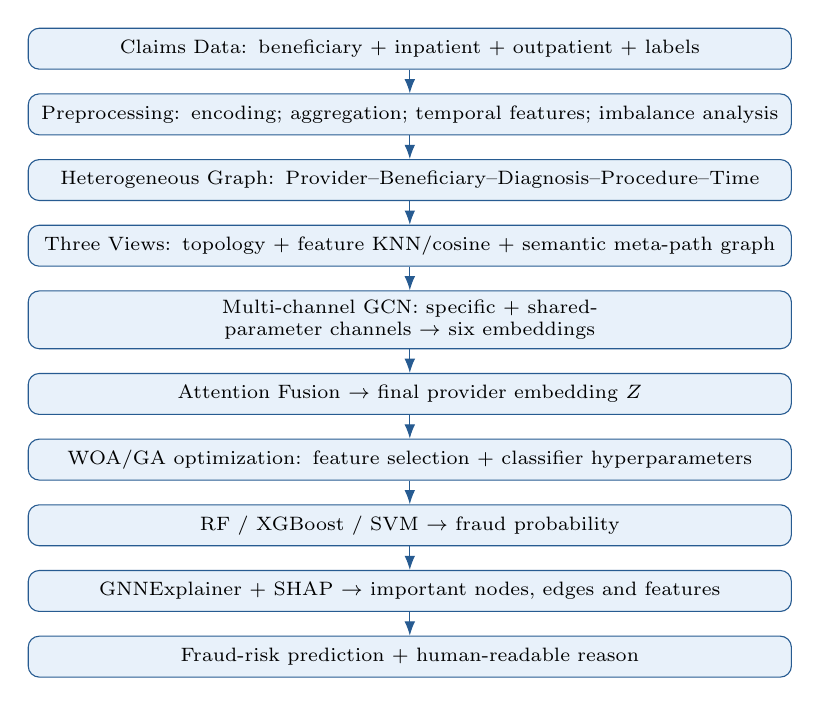
\begin{tikzpicture}[node distance=3mm,box/.style={rectangle,rounded corners,draw=NITBlue,fill=NITLight,align=center,text width=.78\textwidth,minimum height=5.2mm,font=\scriptsize},arrow/.style={-{Latex[length=1.8mm]},draw=NITBlue}]
\node[box](a){Claims Data: beneficiary + inpatient + outpatient + labels};
\node[box,below=of a](b){Preprocessing: encoding; aggregation; temporal features; imbalance analysis};
\node[box,below=of b](c){Heterogeneous Graph: Provider--Beneficiary--Diagnosis--Procedure--Time};
\node[box,below=of c](d){Three Views: topology + feature KNN/cosine + semantic meta-path graph};
\node[box,below=of d](e){Multi-channel GCN: specific + shared-parameter channels $\rightarrow$ six embeddings};
\node[box,below=of e](f){Attention Fusion $\rightarrow$ final provider embedding $Z$};
\node[box,below=of f](g){WOA/GA optimization: feature selection + classifier hyperparameters};
\node[box,below=of g](h){RF / XGBoost / SVM $\rightarrow$ fraud probability};
\node[box,below=of h](i){GNNExplainer + SHAP $\rightarrow$ important nodes, edges and features};
\node[box,below=of i](j){Fraud-risk prediction + human-readable reason};
\foreach \x/\y in {a/b,b/c,c/d,d/e,e/f,f/g,g/h,h/i,i/j}{\draw[arrow](\x)--(\y);}
\end{tikzpicture}\end{frame}

\begin{frame}{Proposed Heterogeneous Graph Construction}
\begin{itemize}
\item \textbf{Target node:} Provider; prediction is Potential Fraud / Non-Fraud.
\item \textbf{Context nodes:} Beneficiary, Diagnosis, Procedure, Time and Claim.
\item \textbf{Relations:} Provider--Beneficiary, Provider--Diagnosis, Provider--Procedure and Provider--Time.
\item \textbf{Topology view:} preserve observed claim relationships.
\item \textbf{Feature view:} KNN edges using cosine similarity between node features.
\item \textbf{Semantic view:} higher-order provider similarity using shared beneficiary, diagnosis, procedure and time patterns.
\end{itemize}\end{frame}

\begin{frame}{Explainable AI -- ``Why Was This Provider Flagged?''}
\begin{columns}[T]
\column{.48\textwidth}\begin{block}{GNNExplainer}
Identifies influential subgraph structure and feature dimensions for a particular GNN prediction.
\end{block}
\column{.48\textwidth}\begin{block}{SHAP}
Quantifies how individual tabular features push the prediction toward fraud or non-fraud.
\end{block}
\end{columns}
\begin{itemize}
\item Example explanation: unusually high claim volume, high reimbursement, concentrated procedure patterns, and strong connections to a small set of beneficiaries/diagnoses contributed to high risk.
\item Graph explanation: show influential neighboring nodes/edges and relation types.
\item Feature explanation: show positive/negative SHAP contributions.
\item Optional counterfactual: identify minimal changes that would move the prediction toward non-fraud.
\end{itemize}\end{frame}

\begin{frame}{Final Proposed Architecture}
\centering
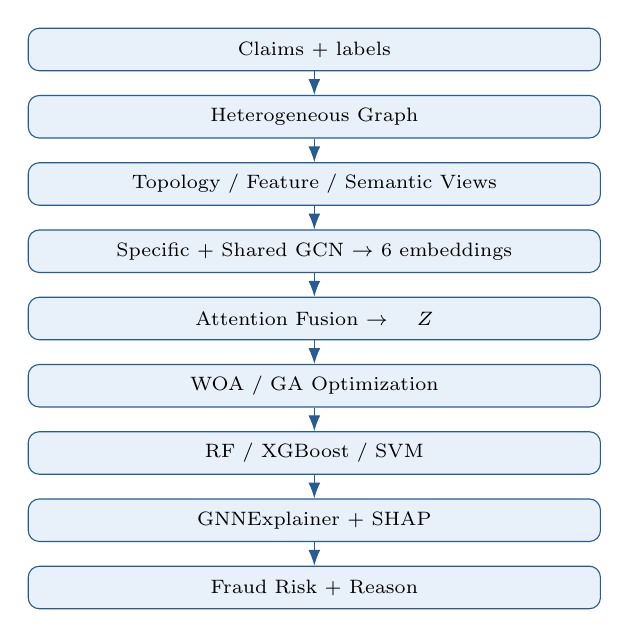
\begin{tikzpicture}[node distance=3mm,box/.style={rectangle,rounded corners,draw=NITBlue,fill=NITLight,align=center,text width=.58\textwidth,minimum height=5.4mm,font=\scriptsize},arrow/.style={-{Latex[length=2mm]},draw=NITBlue}]
\node[box](a){Claims + labels};
\node[box,below=of a](b){Heterogeneous Graph};
\node[box,below=of b](c){Topology / Feature / Semantic Views};
\node[box,below=of c](d){Specific + Shared GCN $\rightarrow$ 6 embeddings};
\node[box,below=of d](e){Attention Fusion $\rightarrow Z$};
\node[box,below=of e](f){WOA / GA Optimization};
\node[box,below=of f](g){RF / XGBoost / SVM};
\node[box,below=of g](h){GNNExplainer + SHAP};
\node[box,below=of h](i){Fraud Risk + Reason};
\foreach \x/\y in {a/b,b/c,c/d,d/e,e/f,f/g,g/h,h/i}{\draw[arrow](\x)--(\y);}
\end{tikzpicture}\end{frame}

\begin{frame}{Revised Objectives}
\begin{enumerate}
\item Develop a heterogeneous graph-based healthcare fraud detection framework inspired by MHGSL.
\item Combine topology, feature-similarity and semantic views using multi-channel GCNs and attention fusion.
\item Integrate WOA/GA-based feature selection and hyperparameter optimization.
\item Compare graph models with SVM, RF, XGBoost and conventional oversampling baselines.
\item Use GNNExplainer and SHAP to provide instance-level reasons for fraud-risk predictions.
\item Evaluate Accuracy, Precision, Recall, F1, ROC-AUC, PR-AUC, confusion matrix and computational cost.
\end{enumerate}\end{frame}

\begin{frame}{Expected Milestones / Work Plan}
\begin{enumerate}
\item Literature + dataset: finalize review and download/understand public dataset.
\item Graph preparation: build provider-centric heterogeneous graph and three views.
\item GCN model: implement specific/shared channels and attention fusion.
\item Optimization: integrate WOA/GA and compare imbalance methods.
\item XAI: implement GNNExplainer + SHAP and generate fraud reasons.
\item Evaluation: ablation, baselines, metrics, scalability and final report.
\end{enumerate}\end{frame}
\end{document}
